
%(BEGIN_QUESTION)
% Copyright 2011, Tony R. Kuphaldt, released under the Creative Commons Attribution License (v 1.0)
% This means you may do almost anything with this work of mine, so long as you give me proper credit

One of the major processes used to treat municipal wastewater is {\it aeration}, where the dissolved oxygen concentration of the wastewater is enhanced by bubbling air through the water in an {\it aeration basin}.  A dissolved oxygen (``DO'') analyzer measures the oxygen concentration in the wastewater, and a controller varies the speeds of blowers pumping air into the basins using AC motors powered through variable-frequency drives (VFDs):

$$\includegraphics[width=15.5cm]{i03291x01.eps}$$

The control strategy used here is called {\it adaptive gain}.  While similar in configuration to feedforward -- where a load variable (in this case, influent flow rate) is used to alter the MV signal going to the final control element(s) of a feedback control loop -- the relay used in this case is a {\it multiplier} rather than the more customary {\it summer} seen in conventional feedforward strategies.

\vskip 10pt

Explain why a multiplying relay really is the most appropriate for this kind of application, ``demonstrating'' your explanation by posing a thought experiment of your own design.

\vfil 

\underbar{file i03291}
\eject
%(END_QUESTION)





%(BEGIN_ANSWER)

This is a graded question -- no answers or hints given!

%(END_ANSWER)





%(BEGIN_NOTES)

Let's perform a thought experiment where the influent flow rate {\it doubles}.  Our question is, how will the demand for air increase?  Based on our knowledge of oxidation (the mass of oxygen required for oxidation being directly proportional to the mass of substance in need of oxidation), we may conclude that the air demand will likewise double.  Thus, the air flow needs to be controlled as a {\it proportion} of the influent flow.

\vskip 10pt

If we were to simply use a summing relay between the AIC and the blower controls, an increase in influent flow rate would indeed add more air to the nozzles, but it would probably not be the right amount.  We need the AIC controller's output to be {\it mulitplied} by any increases in influent flow in order to maintain the proper ratio of influent to oxygen.

A simple thought experiment proves this to be true.  Suppose the influent flow rate jumps up from 25\% to 50\%.  The increased need for airflow into the basin of course would double.  Now let us suppose the influent flow rate jumps up again, this time from 50\% to 100\%.  Once again we would need to double the amount of air flow from before (i.e. {\it four times} the amount of air compared to the original air flow at 25\% influent rate).  If we had a summing block instead of a multiplier, the additional air flow called for by feedforward action would be only 75\%, not the four-fold (400\%) increase we actually need.

%INDEX% Control, strategies: adaptive gain
%INDEX% Control, strategies: feedforward
%INDEX% Process: wastewater aeration (dissolved oxygen control)

%(END_NOTES)


